\chapter{Turbulence}\label{ch:v}
\begin{quote}
   "\emph{When I meet God, I am going to ask him two questions: why relativity? And why turbulence? I really believe he will have an answer for the first}."
   \begin{flushright}
        Werner Heisenberg
   \end{flushright}
\end{quote}
Turbulence is quite an interesting feature arising in fluids. Turbulent flow is fluid motion characterized by chaotic changes in pressure and flow velocity, both spatially and temporally.
\par Turbulence's ability to transport and mix fluid is unparalleled, comparing it to stardard laminar flows. There's not a unique definition of when a fluid becomes turbulent rather than staying in a chill (and much less chaotic) laminar flow.
\par Usually, we say that a flow is turbulent when the Reynolds' number (\ref{eq:reynoldsnumber}) is much larger than 1. Essentially, what happens is that viscosity is no longer able to damp and constrain the fluid motion, which ends up going nuts.
\par Before going through the essential features of turbulence, we shall briefly consider again our naive bubble description, only to find out that what happens is actually much more complex.
\section{Instabilities}
Consider the system depicted in Fig.\ref{fig:bubble}. As the bubble rises, it will have a non-zero vertical velocity. Let's see what this implies.
\par Consider a stratified, ideal, incompressible fluids with no vorticity\,\footnote{Actually, vorticity is divergent on the boundary.} as those shown in Fig.\ref{fig:stratified_fluid}.
\begin{figure}[h!]
    \centering
    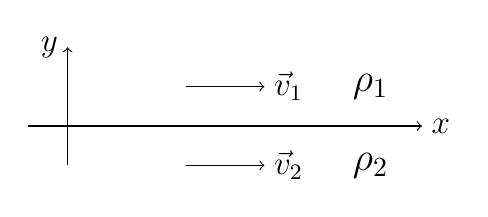
\begin{tikzpicture}
        \draw 
            [->, black] (-2,0)--(3,0) node[anchor=west]{\large $x$};
        \draw 
            [->, black] (-1.5, -0.5)--(-1.5, 1) node[anchor=east]{\large $y$};
        \draw 
            [->, black] (0,0.5)--(1,0.5) node[anchor=west]{\large $\vec{v}_{1}$};
        \draw 
            (2,0.5) node[anchor=west]{\Large $\rho_{1}$};
        \draw 
            [->, black] (0,-0.5)--(1,-0.5) node[anchor=west]{\large $\vec{v}_{2}$};
        \draw 
            (2,-0.5) node[anchor=west]{\Large $\rho_{2}$};
    \end{tikzpicture}
    \caption{Stratified fluids may give raise to instabilities.}
    \label{fig:stratified_fluid}
\end{figure}
Given these assumptions, the velocity fields may be written in terms of a scalar potential
\begin{equation*}
    \vec{v}_{i} = -\nabla\,\phi_{i}
\end{equation*}
Plugging this definition in Euler's equation yields (for example for fluid 1)
\begin{equation*}
    -\nabla(\partial_{t}\phi_{1}) +\nabla\left(\frac{v^{2}}{2}\right) = -\frac{\nabla \,p}{\rho}
\end{equation*}
Let's assume that the scalar potentials are composed of a constant term (temporally speaking) and a small space and time dependent fluctuation
\begin{equation*}
    \phi_{i} = -v_{i}x +\delta\phi_{i}
\end{equation*}
The condition for the fluid to be incompressible then becomes 
\begin{equation*}
    \nabla^{2}\delta\phi_{i} = 0
\end{equation*}
Say that the boundary between the two fluids can be parametrized by $y = \xi(x,t)$, then in the Lagrangian frame we have that 
\begin{equation*}
    \frac{\text{D}\xi}{\text{D}t} = \partial_{y}\delta\phi_{1} = -\partial_{y}\delta\phi_{2}
\end{equation*}
If we assume the pressure to be continuous at the interface and $\delta\phi_{i}$ to be plane waves of the form 
\begin{equation*}
    \delta\phi_{i} = B_{i}\exp(i(kx-\omega t)+k_{y})
\end{equation*}
we're able to find a dispersion relation for the system 
\begin{equation}
    \frac{\omega}{k} = \frac{\rho_{1}v_{1}+\rho_{2}v_{2}}{\rho_{1}+\rho_{2}} \pm \left[-\frac{\rho_{1}\rho_{2}(v_{1}-v_{2})^{2}}{(\rho_{1}+\rho_{2})}\right]^{1/2}
    \label{eq:KHi}
\end{equation}
Unless $v_{1} = v_{2}$, the argument of the square root is always negative, so the oscillation frequency has a purely imaginary component. When you plug that into the plane wave solution, you get an exponentially increasing amplitude for the wave, meaning that the system is unstable.
\par This is called \emph{Kelvin-Helmoltz instability}. The KH instability has characteristic vortices arising, which normally are damped at some point by viscosity, stopping the endless formation of vortices.
\par If we introduce a gravitational field in the vertical direction, we introduce a stabilizing factor in eq.\ref{eq:KHi}
\begin{equation}
    \frac{\omega}{k} = \frac{\rho_{1}v_{1}+\rho_{2}v_{2}}{\rho_{1}+\rho_{2}} \pm \left[\frac{g}{k}\frac{\rho_{2}-\rho_{1}}{\rho_{1}+\rho_{2}}-\frac{\rho_{1}\rho_{2}(v_{1}-v_{2})^{2}}{(\rho_{1}+\rho_{2})}\right]^{1/2}
    \label{eq:KH_RTi}
\end{equation}
Please note that even if $v_{1}=v_{2}$, the system may still be unstable. In fact, in such a scenario, the system is stable only if $\rho_{1}<\rho_{2}$ (referring to Fig.\ref{fig:stratified_fluid}), which actually makes sense: The less dense fluid must float over the denser fluid.
\par Conversely, the fluid is unstable if $\rho_{1}>\rho_{2}$ (\emph{Rayleigh-Taylor instability}). The RT instability presents characteristic "fingers" (or jets) extending from the less dense layer to the denser one.
\section{Properties of Turbulence}
Coming soon.